\documentclass[class=report, crop=false, 12pt,a4paper]{standalone}
\usepackage{enumitem}
\usepackage{float}
\usepackage[normalem]{ulem}
\usepackage{graphicx}
\usepackage{amsmath}
\usepackage{amssymb}
\usepackage{siunitx}
\usepackage{commath}
\usepackage{tikz}
\usetikzlibrary{positioning, fit, calc}   
\tikzset{block/.style={draw, thick, text width=3cm ,minimum height=1.3cm, align=center},   
line/.style={-latex}     
}  
\begin{document}
\section{Lift and drag}
Typical forces of interest for bodies in a flow are \textbf{drag} and \textbf{lift}. We can represent these in dimensionless form:
\begin{gather}
  \textrm{Drag coefficient: }c_D = \frac{F_D}{\frac{1}{2} \rho U_\infty^2S}\\
  \textrm{Lift coefficient: }c_L = \frac{F_L}{\frac{1}{2}\rho U_\infty^2S}
\end{gather}
Where $S$ is a representative area for the body, determined by convention.
\begin{figure}[H]
  \centering
  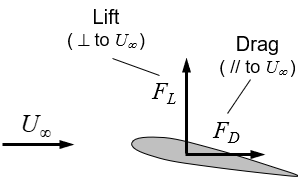
\includegraphics[width = 0.6\textwidth]{../img/diagram9.png}
\end{figure}
\section{Pressure and frictional force distribution}
\begin{figure}[H]
  \centering
  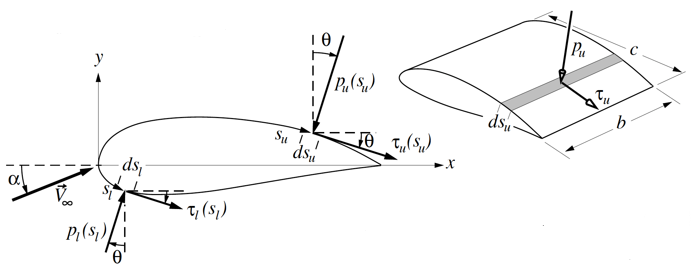
\includegraphics[width = 0.8\textwidth]{../img/diagram10.png}
\end{figure}
\begin{gather}
  L = - \int_{S}^{} \left( p (\hat{n}\cdot \hat{j}) \right)  \,\mathrm{d}S + \int_{}^{S} \left( \vec{\tau} \cdot \hat{j} \right)  \,\mathrm{d}S\\
  D = - \int_{}^{} \left(  p (\hat{n} \cdot \hat{j})\right)  \,\mathrm{d}S  + \int_{}^{} \left(\vec{\tau} \cdot \hat{i} \right)  \,\mathrm{d}S 
\end{gather}
To determine the lift and drag coefficients $c_L$ and $c_D$, we are interested in the pressure distribution over the airfoil, or more specifically in the local pressure difference from the stream pressure $p_{\infty}$.
\begin{equation}
  c_p = \frac{p - p_{\infty}}{\frac{1}{2} \rho V_{\infty}^2}
\end{equation}
Free stream pressure and velocity are $p_\infty$ and $V_\infty$.
\begin{figure}[H]
  \centering
  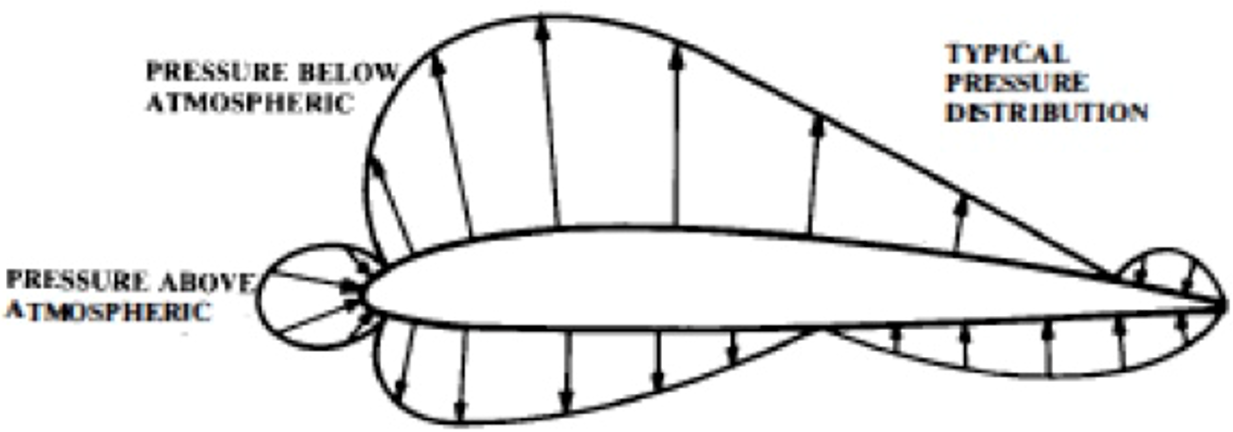
\includegraphics[width = 0.8\textwidth]{../img/diagram11.png}
\end{figure}
\begin{itemize}
  \item Local suction (depression): $c_p < 0$ Vectors point away from the airfoil surface
  \item Local pushing: $c_p > 0$ Vectors point towards the airfoil surface
\end{itemize}
\begin{figure}[H]
  \centering
  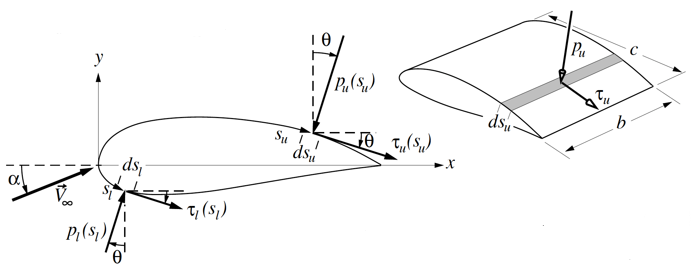
\includegraphics[width = 0.8\textwidth]{../img/diagram10.png}
\end{figure}
\begin{gather}
  L = - \int_{S}^{} \left(p\hat{n}\cdot \hat{j}\right)  \,\mathrm{d}S = \\
  c_L = - \frac{1}{S} \int_{S}^{} \left( \frac{p - p_{\infty}}{\frac{1}{2} \rho V_{\infty}^2} \hat{n} \cdot \hat{j} \right) \,\mathrm{d}S = -\frac{1}{S} \int_{S}^{} \left( c_p \hat{n} \cdot \hat{j} \right)  \,\mathrm{d}S  
\end{gather}
The lift coefficient per unit of span-wise length is:
\begin{equation}
  c_L' - \frac{1}{c}\int_{c}^{0} \left( c_p \hat{n}\cdot\hat{j} \right)  \,\mathrm{d}x 
\end{equation}
\section{Rearrangement of momentum equation - x direction}
\begin{gather}
  \rho \left( u \frac{\partial u}{\partial x} + v\frac{\partial u}{\partial y} \right) = -\frac{\partial p}{\partial x}  + \mu \left( \frac{\partial^2 u}{\partial x^2} + \frac{\partial^2 u}{\partial y^2} \right)\\
  \left(u \frac{\partial u}{\partial x} + v \frac{\partial u}{\partial y} \right) = \left(u \frac{\partial u}{\partial x} + v \frac{\partial u}{\partial y} \right) + v \frac{\partial u}{\partial y} - v \frac{\partial u}{\partial y}\\
  = - v \left(\frac{\partial v}{\partial x} - \frac{\partial u}{\partial y} \right) + \frac{1}{2} \left( \frac{\partial u^2}{\partial x} + \frac{\partial v^2}{\partial x} \right)\\
  = - v \left( \frac{\partial v}{\partial x} - \frac{\partial u}{\partial y} \right) + \frac{1}{2} \frac{\partial}{\partial x} (u^2 + v^2)
\end{gather}
$(u^2 + v^2)$ is the total kinetic energy of the fluid particle. The derivative is the element that takes into the account the variation of this kinetic energy. $\left( \frac{\partial v}{\partial x} - \frac{\partial u}{\partial y} \right)$ relates to the rotation of the particle. This rotation is related to the difference of velocity gradient.
\begin{gather}
  \rho \left[ -v \left( \frac{\partial v}{\partial x} - \frac{\partial u}{\partial y} \right) + \frac{1}{2} \frac{\partial}{\partial x} (u^2 + v^2) \right] = - \frac{\partial p}{\partial x} + \mu \left( \frac{\partial^2 u}{\partial x^2} + \frac{\partial^2 u}{\partial y^2} \right)\\
  - v \left( \frac{\partial v}{\partial x} - \frac{\partial u}{\partial y} \right) = - \frac{\partial}{\partial x} \left( \frac{p}{\rho} + \frac{u^2 + v^2}{2} \right) + \nu \left( \frac{\partial^2 u}{\partial x^2} + \frac{\partial^2 u}{\partial y^2} \right)   
\end{gather}
Our Bernoulli term in the above equation is $\left( \frac{p}{\rho} + \frac{u^2 + v^2}{2} \right)$, gravitational energy is negligible. $\left( \frac{\partial v}{\partial x} - \frac{\partial u}{\partial y} \right)$ is an anti-clockwise rotation. Hence, the vorticity component in the z direction is:
\begin{equation}
  \omega_z = \frac{\partial v}{\partial x} - \frac{\partial u}{\partial y}
\end{equation}
Our final momentum equations in $x$ and $y$ are: 
\begin{gather}
  -v \omega_z = - \frac{\partial}{\partial x} \left( \frac{p}{\rho} + \frac{u^2 + v^2}{2} \right) + \nu \left( \frac{\partial^2 u}{\partial x^2} + \frac{\partial^2 u}{\partial y^2} \right)\\
  u \omega_z = - \frac{\partial}{\partial y} \left( \frac{p}{\rho} + \frac{u^2 + v^2}{2} \right) + \nu \left( \frac{\partial^2 v}{\partial x^2} + \frac{\partial^2 v}{\partial y^2} \right)
\end{gather}
We can make some assumptions:
\begin{itemize}
  \item Inviscid flow - $\nu = 0$ (this may be realistic in some parts of a fluid domain but in real life, inviscid fluids do not exist)
  \item Irrotational flow - $\omega_z = 0$
\end{itemize}
This reduces our equations to:
\begin{gather}
  0 = - \frac{\partial}{\partial x} \left( \frac{p}{\rho} + \frac{u^2 + v^2}{2} \right) + 0\\
  0 = - \frac{\partial}{\partial y} \left( \frac{p}{\rho} + \frac{u^2 + v^2}{2} \right) + 0
\end{gather}
\section{Application of Bernoulli}
\begin{gather}
  p_\infty + \frac{1}{2} \rho V_\infty^2 = p + \frac{1}{2} \rho (u^2 + v^2) = \textrm{constant}\\
  c_p = \frac{p - p_{\infty}}{\frac{1}{2} \rho V_{\infty}^2} = 1 - \frac{u^2 + v^2}{V_\infty^2} = 1 - \frac{||V||^2}{V_\infty^2}
\end{gather}
If $c_p < 0$, $||V|| > V_\infty$ and vice versa. If a fluid particle enters a region where $c_p$ is negative it is accelerated and when $c_P$ is positive it will lose velocity relative to the free stream.
\begin{figure}[H]
  \centering
  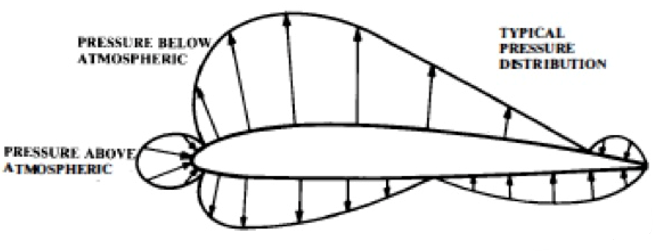
\includegraphics[width = 0.8 \textwidth]{../img/diagram12.png}
\end{figure}
Extending this to 3D, we can derive the 3D vorticity equation. We sum the momentum equations with the assumptions above and take the $ijk$ components as so:
\begin{equation}
  \vec{\omega} = \omega_x \hat{i} + \omega_y \hat{j} + \omega_z \hat{k} = \left( \frac{\partial w}{\partial y} - \frac{\partial v}{\partial z}\right) \hat{i} + \left( \frac{\partial u}{\partial z} - \frac{\partial w}{\partial x}\right) \hat{j} + \left(\frac{\partial v}{\partial x} - \frac{\partial u}{\partial y} \right) \hat{k}
\end{equation}
If $\vec{\omega} = 0$ then a potential function, $\phi(x, y, z)$ exists such:
\begin{equation}
  \begin{cases}
    u = \frac{\partial \phi (x,y,z)}{\partial x}\\
    v = \frac{\partial \phi (x,y,z)}{\partial y}\\
    w = \frac{\partial \phi (x,y,z)}{\partial z}
  \end{cases}
\end{equation}
By plugging in these equations into our continuity equation, we get:
\begin{equation}
  \nabla \cdot \vec{V} = \frac{\partial u}{\partial x} + \frac{\partial v}{\partial y} + \frac{\partial w}{\partial z} = \frac{\partial^2 \phi}{\partial x^2} + \frac{\partial^2 \phi}{\partial y} + \frac{\partial^2 \phi}{\partial z}
\end{equation}
Conservation of momentum (Bernoulli term) is simply:
\begin{equation}
  p + \frac{1}{2} \rho (u^2 + v^2) = \textrm{constant}
\end{equation}
\section{Applicability of irrotational flow}
The flow domain can be subdivided into two parts.
\begin{itemize}
  \item \textbf{Irrotational flow region}, outside of the boundary layer, Bernoulli equation, potential flow and stream function apply.
  \item \textbf{Boundary layer}, layer where all vorticity is confined. The friction shear the airfoil surface acts as a source of vorticity.
\end{itemize}
\begin{figure}[H]
  \centering
  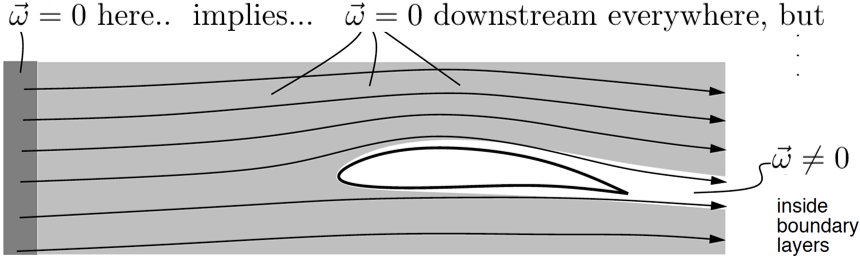
\includegraphics[width = 0.8 \textwidth]{../img/diagram13.png}
\end{figure}
In the case where we consider our fluid inviscid, there is no shear stress being applied on the fluid by the airfoil. We need to understand how the no-slip condition changes. We still need a boundary condition to know the value of $\phi$ in our flow domain.
\section{No-Slip condition for inviscid flow}
Viscous fluid
\begin{equation}
  \nu \neq 0 \rightarrow \vec{V} = 0
\end{equation}
Inviscid flow
\begin{equation}
  \nu = 0 \rightarrow V_n = \vec{V} \cdot \hat{n} = \frac{\partial \phi}{\partial n} = 0
\end{equation}
In essence, with inviscid flow, we are accepting that there is some movement on the boundary, however this is only parallel to the surface. $n$ is the direction orthogonal to the boundary.
\begin{figure}[H]
  \centering
  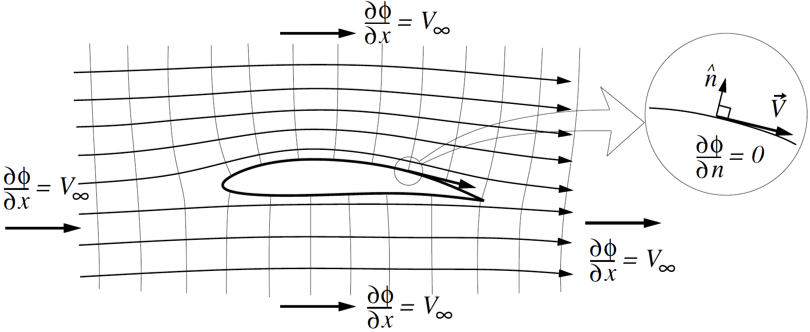
\includegraphics[width = 0.8 \textwidth]{../img/diagram14.png}
\end{figure}
\section{Stream function}
In a 2D flow a stream function, $\psi(x, y)$, can be defined which is always aligned/parallel with the local velocity vector and visualise a streamline. Different streamlines are identified with different values of $\psi (x,y)$
\begin{equation}
  \begin{cases}
    u = \frac{\partial \psi(x,y)}{\partial x}\\
    v = \frac{\partial \psi(x,y)}{\partial y}
  \end{cases}
\end{equation}
Iso-potential lines and streamlines are orthogonal to each other. Streamlines visualise the trajectory of a particle in the field.
\section{Potential flow past bodies}
Flow fields for which an incompressible fluid is assumed to be frictionless and the motion to be irrotational are commonly referred to as \textbf{potential} flows. Paradoxically, potential flows can be simulated by a slow moving, viscous flow between closely spaced parallel plates.
\section{Flow around a corner of arbitrary angle, $\beta$}
Considering a radial coordinate system:
\begin{align}
  \phi &= A r^n \cos(n\theta)\\
  \psi &= Ar^n \sin(n\theta)
\end{align}
\begin{figure}[H]
  \centering
  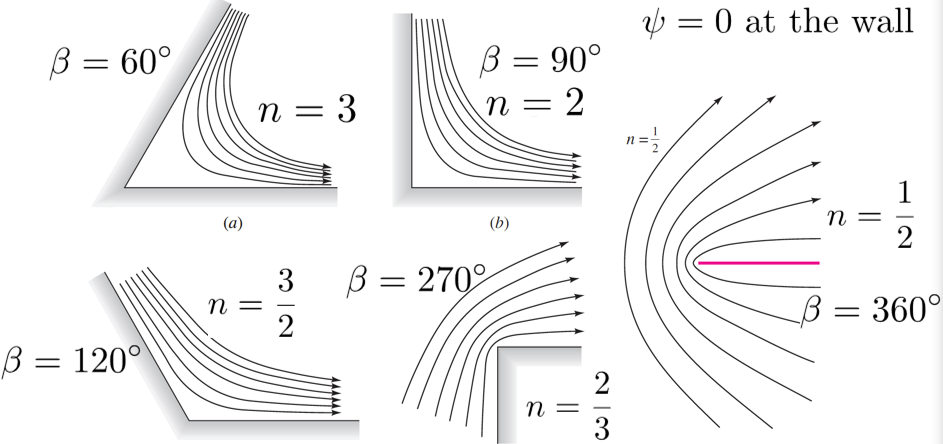
\includegraphics[width = 0.8 \textwidth]{../img/diagram15.png}
\end{figure}
\section{Cylindrical coordinates}
3D vorticity equation:
\begin{gather}
  \vec{\omega} = \omega_r \hat{i}_r + \omega_{\theta} \hat{i}_{\theta} + \omega_z \hat{i}_z\\
  \vec{\omega} = \left(\frac{1}{r}\frac{\partial u_z}{\partial \theta} - \frac{\partial u_{\theta}}{\partial z}\right) \hat{i}_r + \left(\frac{\partial u_r}{\partial z} - \frac{\partial u_z}{\partial r}\right) \hat{i}_{\theta} + \frac{1}{r}\left(\frac{\partial (ru_{\theta})}{\partial r}-\frac{\partial u_r}{\partial \theta}\right)\hat{i}_z
\end{gather}
Potential flow function and stream function:
\begin{equation}
  \textrm{Potential flow}\begin{cases}
    u_r = \frac{\partial \phi}{\partial r}\\
    u_{\theta} = \frac{1}{r}\frac{\partial \phi}{\partial \theta}\\
    u_z = \frac{\partial \phi}{\partial z}
  \end{cases}
  \textrm{Stream function}\begin{cases}
    u_{\theta} = - \frac{\partial \psi}{\partial r}\\
    u_r = \frac{1}{r} \frac{\partial \psi}{\partial \theta}
  \end{cases}
\end{equation}
Conservation of mass (continuity equation):
\begin{equation}
  \nabla \cdot \vec{V} = \frac{1}{r} \frac{\partial (r u_r)}{\partial r} + \frac{1}{r} \frac{\partial u_{\theta}}{\partial \theta} + \frac{\partial u_z}{\partial z} = \frac{\partial^2 \phi}{\partial r^2} + \frac{1}{r}\frac{\partial \phi}{\partial r} +\frac{1}{r^2} \frac{\partial^2 \phi}{\partial \theta^2} + \frac{\partial^2 \phi}{\partial z^2}
\end{equation}
\end{document}